\let\negmedspace\undefined
\let\negthickspace\undefined
\documentclass[journal]{IEEEtran}
\usepackage[a5paper, margin=10mm, onecolumn]{geometry}
%\usepackage{lmodern} % Ensure lmodern is loaded for pdflatex
\usepackage{tfrupee} % Include tfrupee package

\setlength{\headheight}{1cm} % Set the height of the header box
\setlength{\headsep}{0mm}     % Set the distance between the header box and the top of the text

\usepackage{gvv-book}
\usepackage{gvv}
\usepackage{cite}
\usepackage{amsmath,amssymb,amsfonts,amsthm}
\usepackage{algorithmic}
\usepackage{graphicx}
\usepackage{textcomp}
\usepackage{xcolor}
\usepackage{txfonts}
\usepackage{listings}
\usepackage{enumitem}
\usepackage{mathtools}
\usepackage{gensymb}
\usepackage{comment}
\usepackage[breaklinks=true]{hyperref}
\usepackage{tkz-euclide} 
\usepackage{listings}
% \usepackage{gvv}                                        
\def\inputGnumericTable{}                                 
\usepackage[latin1]{inputenc}                                
\usepackage{color}                                            
\usepackage{array}                                            
\usepackage{longtable}                                       
\usepackage{calc}                                             
\usepackage{multirow}                                         
\usepackage{hhline}                                           
\usepackage{ifthen}                                           
\usepackage{lscape}
\begin{document}

\bibliographystyle{IEEEtran}
\vspace{3cm}

\title{1.1.6.27}
\author{EE24BTECH11057 - SHIVAM SHILVANT*
}
% \maketitle
% \newpage
% \bigskip
{\let\newpage\relax\maketitle}

\renewcommand{\thefigure}{\theenumi}
\renewcommand{\thetable}{\theenumi}
\setlength{\intextsep}{10pt} % Space between text and floats


\numberwithin{equation}{enumi}
\numberwithin{figure}{enumi}
\renewcommand{\thetable}{\theenumi}


\textbf{Question}:\\
Prove that the three points $\brak{-4, 6, 10}$, $\brak{2, 4, 6}$ and $\brak{14, 0, -2}$ are collinear.\\ 
\textbf{Solution: }\\
    \begin{table}[h!]    
      \centering
      \begin{tabular}{|c|c|} 
        \hline
        \textbf{Column-I} & \textbf{Column-II} \\
        \hline
        P. Zirconia & 1. Ultra-hard material \\
        \hline
        Q. Cubic boron nitride & 2. High temperature superconductor \\
        \hline
        R. Hafnium carbide & 3. Transformation toughening\\
        \hline
        S. Yttrium aluminium garnet & 4. Ultra-high temperature material \\
        \hline
         & 5. Host material for laser \\
        \hline
          & 6. Micro-crack toughening \\
        \hline
    \end{tabular}
      \caption{}
    \end{table}\\
If the rank of a matrix $M$ is 1, then the points A,B,C are collinear. 
    \begin{align}
        Rank\brak{M} = 1\label{eq1.1.6.22.1}
    \end{align}
Computing matrix $M$
    \begin{align}
        M = \myvec{6 & -2 & -4 \\ 18 & \ -6 & -12}
        \xleftrightarrow[]{R_2 \rightarrow {R_2-3R_1}}  \label{eq1.1.6.22.2}
        \myvec{6 & -2 & -4 \\ 0 & 0 & 0}
    \end{align}
Thus we can conclude that the rank of matrix $M$ is 1 and thus $A,B,C$ are collinear. \\i.e.the given points are collinear.\\
    \begin{figure}[h]
        \centering
       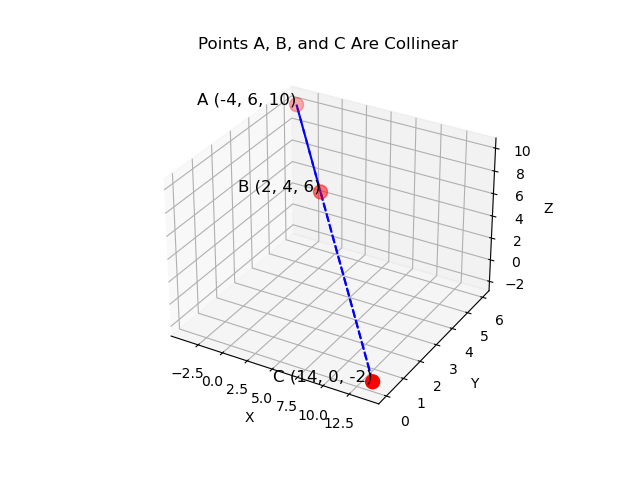
\includegraphics[width=0.7\linewidth]{figs/fig1.png}
       \caption{}
       \label{graph}
    \end{figure}

\end{document} 
